\documentclass[11pt]{article}

\usepackage[margin=0.75in]{geometry}
\usepackage{url}
\usepackage{graphicx}
\usepackage{float}
\graphicspath{ {figs/} }

\title{Finding Gene Signatures Unique to Benzene Exposure}
\author{
  Courtney Schiffman
  \and
  Partow Imani
  \and
  Rebecca Hyde
  \and
  Nima Hejazi
}

\date{December 10, 2015}
\bibliographystyle{siam}

\begin{document}

\maketitle

\abstract{Current U.S. standards allow occupational exposure to benzene at a level of less than 1 ppm. However, there is a concern that even an exposure to benzene at this level has detrimental health effects, and can cause differential expression of various genes. As part of an ongoing study with Martyn Smith�s Superfund Research Program at UC Berkeley, mRNA was collected from Chinese factory workers who had been exposed to various levels of benzene. Initial gene expression analysis showed that a subset of genes from the subjects were differentially expressed between exposed and control subjects in the study. After further analysis, it is hypothesized that it takes only certain pairs of these differentially expressed genes to predict with relative accuracy whether a subject has been exposed to benzene at the less than 1 ppm level. Furthermore, there seem to be several pairs of genes which can act as benzene biomarkers: AQP9 and ACSL1, NFKB1 and IFNB1, PRG2 and ACSL1 , PRG2 and CLEC5A, NFKB1 and CLEC5A, ACSL1 and CLEC5A. In order to help determine whether these gene signatures are unique to benzene exposure, we test whether these same pairs of genes are differentially expressed in other exposure studies, and see whether these genes can act as biomarkers for other confounding exposure/disease and lifestyle variables. To test these genes� sensitivity to other exposure variables, we used data from several  human peripheral blood mononucleocyte cell (pbmc) studies, with mRNA from case and control subjects sequenced by various microarray platforms . While in most cases the genes were very poor predictors of exposure to the various chemicals/lifestyles/diseases, in one exposure case, occupational vs. environmental exposure to nickel, certain pairs of the genes of interest predicted exposure almost perfectly.}

\section{Introduction}

From the benzene study analysis, we take as given the six pairs of differentially expressed genes found to be proposed biological markers of benzene exposure. Our goal is to research whether these genes are unique signatures for benzene, or if their remarkable ability to predict benzene exposure is possibly being cofounded with another exposure, lifestyle, or disease variable. To answer this question, our research extended to six human PBMC datasets, each studying six different exposure, lifestyle, or disease effects on gene expression: exposure to nickel, exposure to arsenic, smoking, stress, peripheral arterial disease and rheumatoid arthritis. For each of these six additional PBMC studies, let $Y$ be an n x 1 binary �treatment� variable indicating exposure, lifestyle, or disease status for each subject within the study. Let $X$ be an n x 2 matrix of gene expression levels, where $n$ is the number of subjects in the study, and where each row of $X$ is the expression levels of two genes for a particular subject in the study.  Since there are six pairs of genes of interest, there will be six different n x 2 matrices $X$ for each study, $X_{1}, ..., X_{6}$, each time changing which two different genes make up the columns of the $X$ matrix. In each study on exposure, lifestyle, or disease, our parameter of interest is the expected value of the binary outcome variable given the gene expression matrix $X_{i}$, $E[Y | X_{i}]$, $i = 1, ..., 6$. In other words, our goal is to estimate $P(Y=1 | X_{i})$, $i = 1, ..., 6$. To put it in a prediction framework, our goal is to build a predictor of the binary treatment variable based on the expression levels of two genes, for various pairs of genes. We then assess the performance of each of the six binary predictors for each of the six studies by estimating the area under the ROC curves. Pairs of genes which are good predictors of exposure, lifestyle, or disease status will have predictor functions with large AUC estimates. The final step is to compare these AUC estimates with the corresponding AUC estimates for the predictors from the study on benzene exposure. We are hoping that at least one of the six pairs of genes does a poor job of predicting exposure, lifestyle, or disease in all of the PBMC studies, and is thus a unique biomarker for benzene exposure in so far as these six datasets are concerned.

\section{Data}

The study of the effect of benzene exposure on health and gene expression began with the collection of DNA from several hundred Chinese factory workers who were exposed to various levels of benzene in the factory environment. In this study, a lower than 1 ppm level was chosen to be the exposure level of interest because this is the relevant level of exposure for workers in the United States (assuring that any results from our work would have implications for health policy). Furthermore, the sample size of workers who were exposed to benzene at levels higher than less than 1 ppm was considerably smaller. This left 77 workers who were control subjects or exposed to benzene at a level of less than 1 ppm. First, differential expression analysis was done using microarray expression levels. A subset of genes were identified to be differentially expressed between exposure and control subjects. Next, to confirm this technology and the differential expression of these genes, the \textit{nCounter} digital counting technology (Nanostring Technologies) was used to sequence the mRNA of the subjects. The results of the \textit{nCounter} technology confirmed the microarray expression levels and differential expression analysis. All subsequent analysis focused on a subset of 33 differentially expressed genes found in the microarray study. However, in this paper the differential expression analysis and treatment prediction done for the benzene data set used the count data from the nCounter technology, rather than the microarray expression levels. Therefore, we focused on the genes selected from the microarray study as differentially expressed, but the actual data we used was provided by the Nanostring sequencing technology. The Nanostring data was normalized to positive control genes and the geometric mean of three housekeeping genes (B2M, RPLPO, PGK1). 

Although it is beyond the scope of this paper, in order to fully understand the chosen structure of the data (i.e. the n x 2 design matrix $X$), it is worth noting how subsetting the data further into just six pairs of genes in order to predict benzene exposure with relative accuracy was determined: The Super Learner meta-learning algorithm and \textit{cvAUC} (Cross Validated Area Under the Curve) packages in R [cite CRAN] were used to identify that only two genes were necessary to build a predictor of benzene exposure with an estimated area under the ROC curve of around ninety to ninety-five percent. SuperLearner was again used to identify the specific pairs of genes which are biomarkers of benzene exposure. Because several genes showed up in more than one pair, there are in total only six distinct genes in the final data set, identified by common gene symbols.

The public PBMC datasets were all obtained from the Gene Expression Omnibus (GEO) repository. We used processed and normalized data sets, which were available for each study, therefore using perfectly reproducible data. All of the PBMC data sets were from various microarray platforms, and each study employed a series of normalization steps, using R packages such as \textit{SCAN} (Single Channel Array Normalization), \textit{affy} (Robust Multichip Average method), \textit{COMBAT}, and \textit{affyPLM}, and other normalization methods such as full quantile normalization. Manufacturer gene identifiers were then mapped to common gene symbols in order to identify the genes needed for the six pairs of genes in the analysis. Annotation packages specific to each microarray platform were found (from the Bioconductor website) and used to perform gene ID mappings. However, in many cases these mappings were not unique, and several different manufacturer IDs were mapped to the same common gene symbol. For example, in the smoking PBMC data set, all of the platform gene IDs 211743-s-at, 212012-at, 212013-at, and 220798-x-at mapped to the PRG2 gene. Therefore, in each of these cases, all genes that mapped to the same gene symbol in the benzene data were included, and the analysis were run separately for each duplicate of the gene, since it was not possible to identify which gene variant exactly corresponded to the appropriate gene in the benzene study. Because there are several candidates for certain genes, to simplify the final results, we recorded the largest  AUC estimate from all of the gene replicate candidates. For example, if there were two possible genes that mapped to the common gene symbol of AQP9, we ran the analysis on both genes paired with the gene mapping to ACSL1, and picked the largest cvAUC value to report in the results that follow.


\section{Methods}

\subsection{\textit{Limma} and Differential Expression Analysis}

Before building predictor functions of exposure for each data set and pair of genes, we conducted a differential expression analysis for the six pbmc studies to see if any of the genes in the pairs of interest were differentially expressed across control and exposed subjects. Recall that all of the pbmc studies were done using various single channel microarray platforms, therefore, we used the popular \textit{Limma} package in R to do the differential expression analysis. The differential expression analysis is performed in two steps. The first step fits a linear model to each gene, assuming that the expected expression of the gene is a linear function of, in our case, two covariates because of the simple two-group design matrix. For the linear model fit to each gene, the design matrix is n x 2 in dimension, where $n$ is the number of subjects, and the outcome variable is an n x 1 vector of the gene�s expression in each subject. The first column of the design matrix is all ones (representing the intercept), and the second column is a zero-one vector indicating treatment or control status for each subject. Therefore, the second coefficient is the coefficient of interest, since it represents the difference between treatment/exposure and control effects. Once this coefficient (and its variance)  is estimated for each gene, the second step is to shrink the estimated variances of each coefficient, and then divide the coefficient by this new smaller standard error to get a t-statistic. To get the new, smaller variance estimate, first a prior distribution on the unknown variances is assumed. This prior distribution sheds light on how the variances of the contrast coefficients change from gene to gene, and therefore incorporates the relationship of all of the thousands of genes into the parametric model. This prior distribution is how \textit{Limma} uses information from all of the genes to create more accurate differential expression measures. Conditioning on the observed empirical variance of each coefficient and using the assumed prior, the posterior mean of the distribution of the variances replaces the empirical variance for each coefficient�s t-statistic. Because of the form of the specified priors, the variances of genes that have small observed residual degrees of freedom from the linear model relative to the prior degrees of freedom get shrunk toward the prior values more.

There are several assumptions made in the \textit{Limma} package in regard to the distribution of the contrast coefficients and their variances. For every gene $j$, the contrast coefficient is assumed to be normally distributed, with expected value $E(\hat{\beta}_{j} | \beta_{j}) = \beta _{j}$ and variance given by the second diagonal entry of the covariance matrix $C^{T} V_{j} C \sigma_{j}^{2}$. For the empirical Bayes method, the contrast coefficients for each gene are assumed to be independent. Furthermore, the resulting t-statistic, after the shrinking of the estimated variance using the empirical Bayes method, is assumed to follow a t-distribution under the null hypothesis that each contrast coefficient is equal to zero. The chi-square distribution is the prior distribution assumed for the variance parameters, and a prior normal distribution is assumed for the contrast coefficients of genes that are not differentially expressed. As for the validity of these assumptions, it is difficult to test the prior distributional assumptions on the coefficients and their variances, which is problematic because the t-distribution of the final moderated statistic, and therefore our conclusions about differential expression, rely on these marginal distribution assumptions. For the independence assumption, it seems unlikely that the coefficients would be independent of one another, since gene relationships are highly complex. Therefore, although the \textit{Limma} package and its methods are popular and widely used, they do involve a troubling set of assumptions.


\subsection{The Super Learner Algorithm and \textit{cvAUC}}

The Super Learner algorithm is a meta-learning algorithm that makes use of a library of machine learning algorithms to produce an ensemble model composed of weighted components (with each component being an algorithm in the original library), using cross-validation in order to achieve optimal prediction. For a given loss function -- in our case of binary prediction, the squared error loss and negative log loss functions, or a convex combination of the two, are both appropriate -- the Super Learner algorithm trains the machine learning algorithms in the library on all but one of the specified folds, determining the risk associated with each algorithm by the performance prediction on the remaining fold (i.e., the test set). Each of the algorithms that are assembled into the ensemble model are weighted such that the algorithm with the lowest risk is given the highest weight (i.e., algorithms are weighted in ascending order of associated risk). This process is performed with each fold being treated as a test set, with the final weights in the ensemble model produced by combining the risks across all runs of the Super Learner algorithm. The cvAUC method is used to build off of the Super Learner algorithm by determining the area under the curve (AUC) associated with the receiver operating characteristic (ROC) curve for the classification in each of the different binary outcome cases. 

Within the scope of this analysis, the Super Learner meta-algorithm is used to predict the exposure class labels for each of the PBMC classes. The library used in the various runs of Super Learner included logistic regression (via SL.glm), stepwise AIC-based model selection (via SL.stepAIC), Bayesian generalized linear regression (via SL.bayesglm), random forests for binary classification (via SL.randomForest), general additive models (via SL.gam), and mean-based classification (via SL.mean). The Super Learner algorithm was run on design matrices that included each of the pairs of genes included in our analyses, with the exposure label predicted for each exposure in the PBMC data sets considered (that is, benzene, nickel, PAD, smoking, arsenic, stress, and arthritis). The AUC for each ROC curve was computed for the classification produced by Super Learner in each of the exposure and gene pair combinations. The use of the \textit{cvAUC} package allowed for computationally efficient estimation of the AUC using an approach based on influence curves, and the AUC estimates were then used to assess the quality of prediction offered by each of the gene pairs of interest for each of the six types of exposure present in the PBMC data sets considered.



\subsection{LASSO Regression and Comparisons with Super Learner}

In order to validate the effectiveness of Super Learner for the given problem, we aim to compare its results to those acquired by a simpler prediction model, such as the least absolute shrinkage and selection operator (LASSO). LASSO is a shrinkage and selection method for linear regression, which penalizes the $L_{1}$ norm of the coefficient matrix, given a constraint $\lambda$. All six of the genes of interest were used to create the scaled design matrix, since our goal was to see if LASSO would choose a pair of genes from the pairs of genes that Super Learner selected. In other words, we hoped that as the penalty increased, and as the LASSO dropped covariates, the last two covariates (genes) would be among one of our defined pairs of interest. In order to choose the optimal $\lambda$, via the mean squared error (MSE) of the LASSO for a range of $\lambda$ values, the value of $\lambda$ which minimized the mean squared error was selected. We then obtained the coefficient matrix returned by LASSO for that chosen value of $\lambda$. The key assumption that LASSO makes is that the expected value of the outcome given the covariates is linear with respect to the covariates. This is a stronger parametric assumption than the assumptions made when using the Super Learner meta-learning algorithm. Here, we are restricted to a linear model, whereas in the use of Super Learner, we have the freedom of using a variety of machine learning algorithms, with varying degrees of bias, variance, and parametric assumptions. However, we conclude that LASSO may be a promising algorithm to use in a problem of this nature because the covariates -- the six genes of interest -- are most likely correlated to a certain (though unknown) extent, and the LASSO will help to minimize the noise induced by this possible correlation structure.

\section{Results}

Tables 1, 2, and 3 show the estimated differential expression measures of the genes ACSL1, AQP9, NFKB1, IFNB1, CLEC5A, and PRG2 for the benzene, smoking, and nickel data sets, respectively. The ratio value in the differential expression tables for both the benzene and PBMC studies is the log2 fold change in expression values between the treatment and control groups. As seen in Table 1, all six genes are estimated to be differentially expressed in the benzene study, which is not surprising since they were originally chosen for this reason. As seen in Table 3, five out six genes were differentially expressed for nickel, the exception being CLEC5A. None of the six genes from the PAD, smoking, arsenic, and stress data sets were found to be differentially expressed. The results for smoking can be seen in Table 2. Note that the differential expression tables for arsenic, PAD, and stress data sets were not included in this paper, although they show similar results to the smoking data set.

Table 4 shows the AUC values for the relevant combinations of differentially expressed genes for benzene and the PBMC studies. The AUC values for benzene are high, ranging from $0.91$ to $0.94$. AUC values for nickel are also high, ranging from $0.75$ to $1.00$. The remaining AUC ranges are as follows: PAD: $0.22$ to $0.73$, smoking: $0.26$ to $0.69$, arsenic: $0.15$ to $0.50$, stress: $0.26$ to $0.39$, and arthritis: $0.29$ to $0.71$.

Figures 1 and 2 show the ROC curves for benzene for ACSL1 with AQPN and NFKB1 with IFNB1. Figures 3 and 4 show the ROC curves for nickel for ACSL1 with AQP9 and PRG2 with CLEC5A. Figures 5 and 6 show the ROC curves for smoking for ACSL1 with CLEC5A and PRG2 with CLEC5A. 

The final pair of genes left in the prediction model when using LASSO on the benzene data set were ACSL1 and AQP9. When finding the optimal lambda by minimizing mean squared error, the resulting model has a non-zero coefficient only for ACSL1. The AUC values returned for the LASSO model with ACSL1 and AQP9 was $0.8842975$, while the AUC value for the regression with LASSO�s optimal fit, containing just ACSL1, was $0.8836088$. Building a Super Learner predictor for this same pair and just IFNB1 gave AUC values of $0.9113095$ and $0.9138095$, respectively.  


\section{Discussion}

\subsection{Conclusions}

Based on the AUC values for the six pairs of genes in Table 4, the optimal pair for benzene detection is ACSL1 and AQP9. This is because, while other pairs such as IFNB1 with NFKB1, and PRG2 with ACSL1 had slightly higher AUC values for predicting benzene exposure, the corresponding AUC values for prediction of nickel exposure were also very high, $0.85$ and $0.90$ respectively.  The nickel AUC value for ACSL1 and AQP9 is $0.75$, which was the lowest nickel AUC value. The other five PBMC exposures did not have high AUC values for ACSL1 with AQP9, so they do not pose a conflict. In addition, the LASSO analysis also returned ACSL1 and AQP9 as the optimal pair, showing that our estimation of this gene pair as the optimal gene pair is robust to choosing simpler parametric models as predictors of exposure.

\subsection{Further Questions}

There are many biological questions that still need to be addressed, but first a few additional statistical questions will be mentioned. Since SuperLearner plays such a key role in the statistical analysis of this project, the learners chosen to build the SuperLearner library should be studied further. For example, how robust is the prediction function to the choice of learners? Other learners should be added to the model, and perhaps some custom built learners as well, to study the impact on the prediction function. Another question which needs to be addressed is the method used to determine the differential expression of the genes in the PBMC data sets. For example, in the nickel data set, using the \textit{Limma} package to assess differential expression results in many genes being found to be differentially expressed across the subjects who experienced occupational or environmental exposure to nickel. One possible explanation for this is that the nickel refinery factory workers were exposed to such high levels of nickel that it caused many of their gene expressions to change, including our genes of interest. However, to support the differential expression findings from using \textit{Limma}, other differential expression methods should be explored and tested.

Another question that is not addressed in this project is whether these target genes are found to be differentially expressed in humans, or other species, in other studies involving benzene exposure. A further arm of this project should involve studying other genetic datasets where subjects have been exposed to benzene, to ensure that these same genes are still differentially expressed, and, ideally, predict benzene exposure well. Furthermore, while the investigation of six exposure data sets is a good start to exploring whether these pairs are unique biomarkers to benzene, one could argue that more research is needed to continue to explore other common exposures/lifestyles/diseases which might be confounding the results. Related to this point, a good place to start with this is to investigate other common exposures the Chinese factory workers were experiencing in their occupations. Are those who are exposed to benzene also commonly exposed to other toxins? Are there common diseases within this population which should be focused on? Are there common lifestyles, diets, or habits?

Given the ability of many of these pairs of genes to predict nickel exposure, the nickel study (GSE40392) should be researched further. Were the nickel refinery workers also exposed to benzene? If so, this could be why the pairs of genes of interest predicted nickel exposure. Another explanation is that nickel and benzene have some kind of biological connection in terms of their effect on the human body. Perhaps the fact that exposures to both toxins can be predicted by the same genes can illuminate our understanding of each toxin separately, and we can learn more about each toxin than if they were studied in isolation. To aid in the understanding of each toxin?s effect on the body, the annotation of these six genes (AQP9. ACSL1, NFKB1, IFNB1, PRG2, CLEC5A) should be studied, focusing on their molecular functions, which biological processes they are involved in, which previous studies have focused on them, and their relationship to one another. To explore this, resources such as the Gene Ontology Consortium should be utilized, as well as Gene Ontology tools such as \textit{AmiGO}. The relationships and functions discovered through this gene ontology research could potentially help to support the statistical findings of this paper and provide further evidence that these genes can accurately predict benzene exposure. Furthermore, the gene ontology research would hopefully support that these genes are unique biomarkers to benzene, and are not, for example, just common genes which react to inflammation and could easily be reacting to a variety of different exposures. \nocite{*}

\bibliography{group_report}

\newpage
\appendix

\section{TABLES AND FIGURES}

\begin{table}[ht]
	\caption {Differential expression in benzene exposure} \label{tab:benzene} 
	\centering
		\begin{tabular}{rlrrr}
  			\hline
 			Gene & Ratio & P-value & Q-value \\ 
  			\hline
			ACSL1 & 1.86 & 0.00 & 0.00 \\ 
  			AQP9 & 2.44 & 0.00 & 0.00 \\ 
  			CLEC5A & 2.39 & 0.00 & 0.00 \\ 
  			IFNB1 & 3.06 & 0.00 & 0.00 \\ 
  			NFKB1 & 1.64 & 0.00 & 0.00 \\ 
  			PRG2 & 1.67 & 0.01 & 0.02 \\ 
   			\hline
		\end{tabular}
\end{table}

\begin{table}[ht]
		\caption {Differential expression in smoking exposure} \label{tab:smoking} 
		\centering
		\begin{tabular}{rrrrrr}
 		 	\hline
 			& logFC & AveExpr & t & P.Value & adj.P.Val \\ 
 			 \hline
			PRG2 & 0.12 & 4.49 & 1.04 & 0.31 & 1.00 \\ 
  			AQP9 & 0.18 & 7.56 & 0.62 & 0.54 & 1.00 \\ 
  			NFKB1 & 0.14 & 8.01 & 0.61 & 0.54 & 1.00 \\ 
  			ACSL1 & -0.27 & 6.71 & -0.58 & 0.56 & 1.00 \\ 
  			CLEC5A & -0.12 & 4.43 & -0.52 & 0.61 & 1.00 \\ 
  			IFNB1 & -0.02 & 4.49 & -0.13 & 0.90 & 1.00 \\ 
  			\hline
		\end{tabular}
\end{table}

\begin{table}[ht]
	\caption {Differential expression in nickel exposure} \label{tab:nickel} 
	\centering
	\begin{tabular}{rrrrrr}
 			\hline
 			& logFC & AveExpr & t & P.Value & adj.P.Val \\ 
  			\hline
			NFKB1 & 1.11 & 9.65 & 5.63 & 0.00 & 0.00 \\ 
  			ACSL1 & 0.88 & 9.47 & 4.92 & 0.00 & 0.00 \\ 
  			PRG2 & -0.48 & 5.32 & -4.42 & 0.00 & 0.00 \\ 
  			IFNB1 & -0.41 & 3.83 & -3.93 & 0.00 & 0.00 \\ 
  			AQP9 & 1.02 & 9.53 & 3.70 & 0.00 & 0.00 \\ 
  			CLEC5A & -0.11 & 5.88 & -0.85 & 0.40 & 0.47 \\ 
  			 \hline
	\end{tabular}
\end{table}


\begin{table}[H]
		\caption{AUC estimates for all exposures (via Super Learner \& cvAUC)} \label{tab:auc}
		\begin{center}
		\tabcolsep=0.15cm
		\scalebox{1.1}{
		\begin{tabular}{rlllllll}
  			\hline
 			& Benzene & Nickel & PAD & Smoking & Arsenic & Stress & Arthritis \\ 
 		 	\hline
			ACSL1 \& AQP9 & 0.9113095 & 0.75 & 0.5935673 & 0.5307692 & 0.1785714 & 				0.3397516 & 0.2944444 \\ 
  			NFKB1 \& IFNB1 & 0.939881 & 0.85 & 0.2251462 & 0.2653846 & 0.3285714 & 				0.3847826 & 0.437037 \\ 
  			PRG2 \& ACSL1 & 0.9204762 & 0.9 & 0.7339181 & 0.6615385 & 0.4666667 & 					0.3745342 & 0.3555556 \\ 
  			PRG2 \& CLEC5A & 0.9382143 & 1 & 0.5204678 & 0.6846154 & 0.5 & 0.3888199 & 			0.7148148 \\ 
  			NFKB1 \& CLEC5A & 0.9057143 & 0.8625 & 0.2704678 & 0.5769231 & 0.2428571 & 			0.2664596 & 0.6740741 \\ 
  			ACSL1 \& CLEC5A & 0.9150595 & 0.8375 & 0.6842105 & 0.6923077 & 0.15 & 					0.3409938 & 0.6703704 \\ 
   			\hline
		\end{tabular}
		}
		\end{center}
\end{table} 

\begin{figure}[H]
		\centering
		\caption{ROC CURVES FOR BENZENE STUDY FOR ACSL1 AND AQP9}
	 	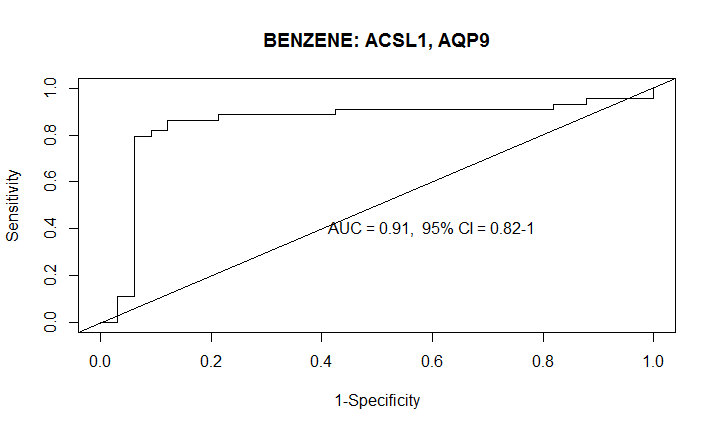
\includegraphics[scale=0.60]{../paper/figs/benzene1.png}
\end{figure}

\begin{figure}[H]
		\centering
		\caption{ROC CURVE FOR BENZENE STUDY WITH NFKB1 AND IFNB1}
	 	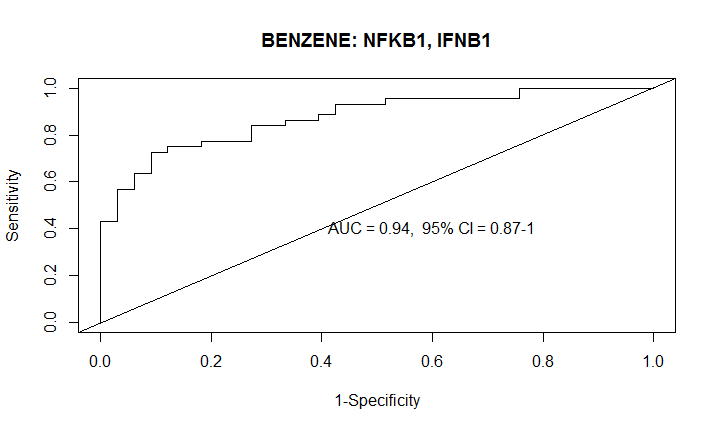
\includegraphics[scale=0.60]{../paper/figs/benzene2.png}
\end{figure}

\begin{figure}[H]
		\centering
		\caption{ROC CURVES FOR NICKEL FOR ACSL1 AND AQP9}
	 	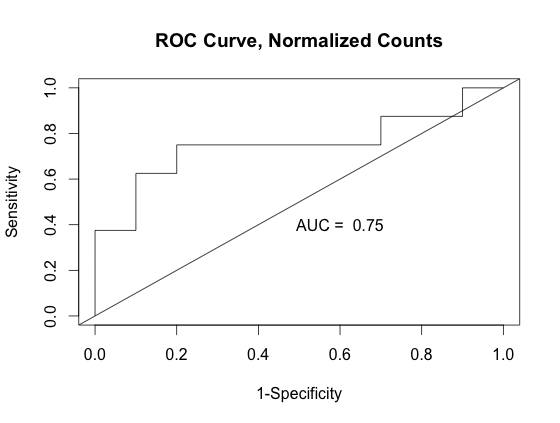
\includegraphics[scale=0.65]{../paper/figs/Nickel_ASCL1-APQ9.png} 
\end{figure}

\begin{figure}[H]
		\centering
		\caption{ROC CURVES FOR NICKEL FOR PRG2 AND CLEC5A}
	 	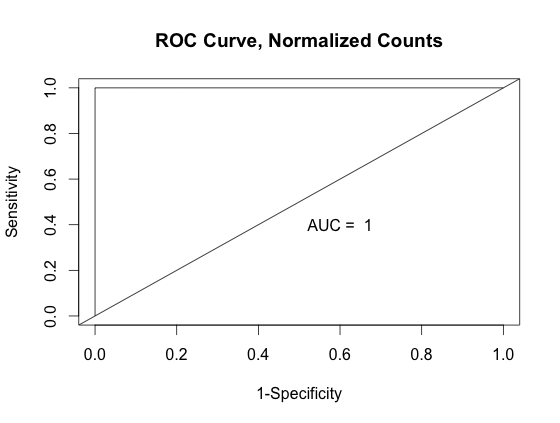
\includegraphics[scale=0.65]{../paper/figs/Nickel_PRG2-CLEC5A.png} 
\end{figure}

\begin{figure}[H]
		\centering
		\caption{ROC CURVES FOR SMOKING WITH ACSL1 AND AQP9}
	 	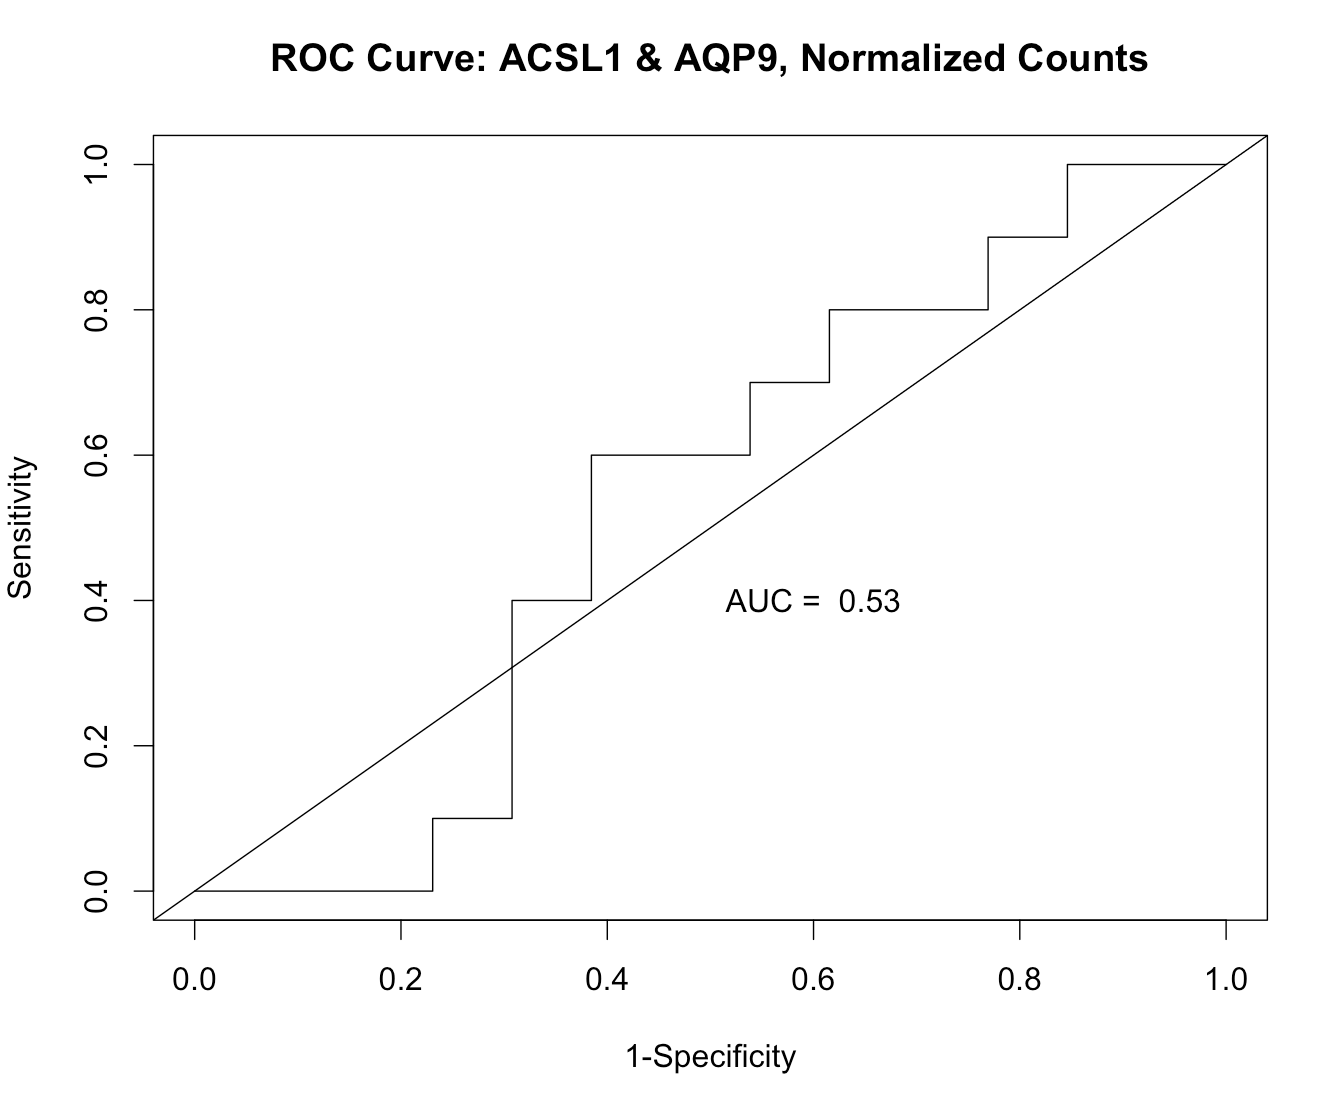
\includegraphics[scale=0.50]{../paper/figs/smoking3.png}
\end{figure}

\begin{figure}[H]
		\centering
		\caption{ROC CURVES FOR SMOKING WITH CLEC5A AND ACSL1}
	 	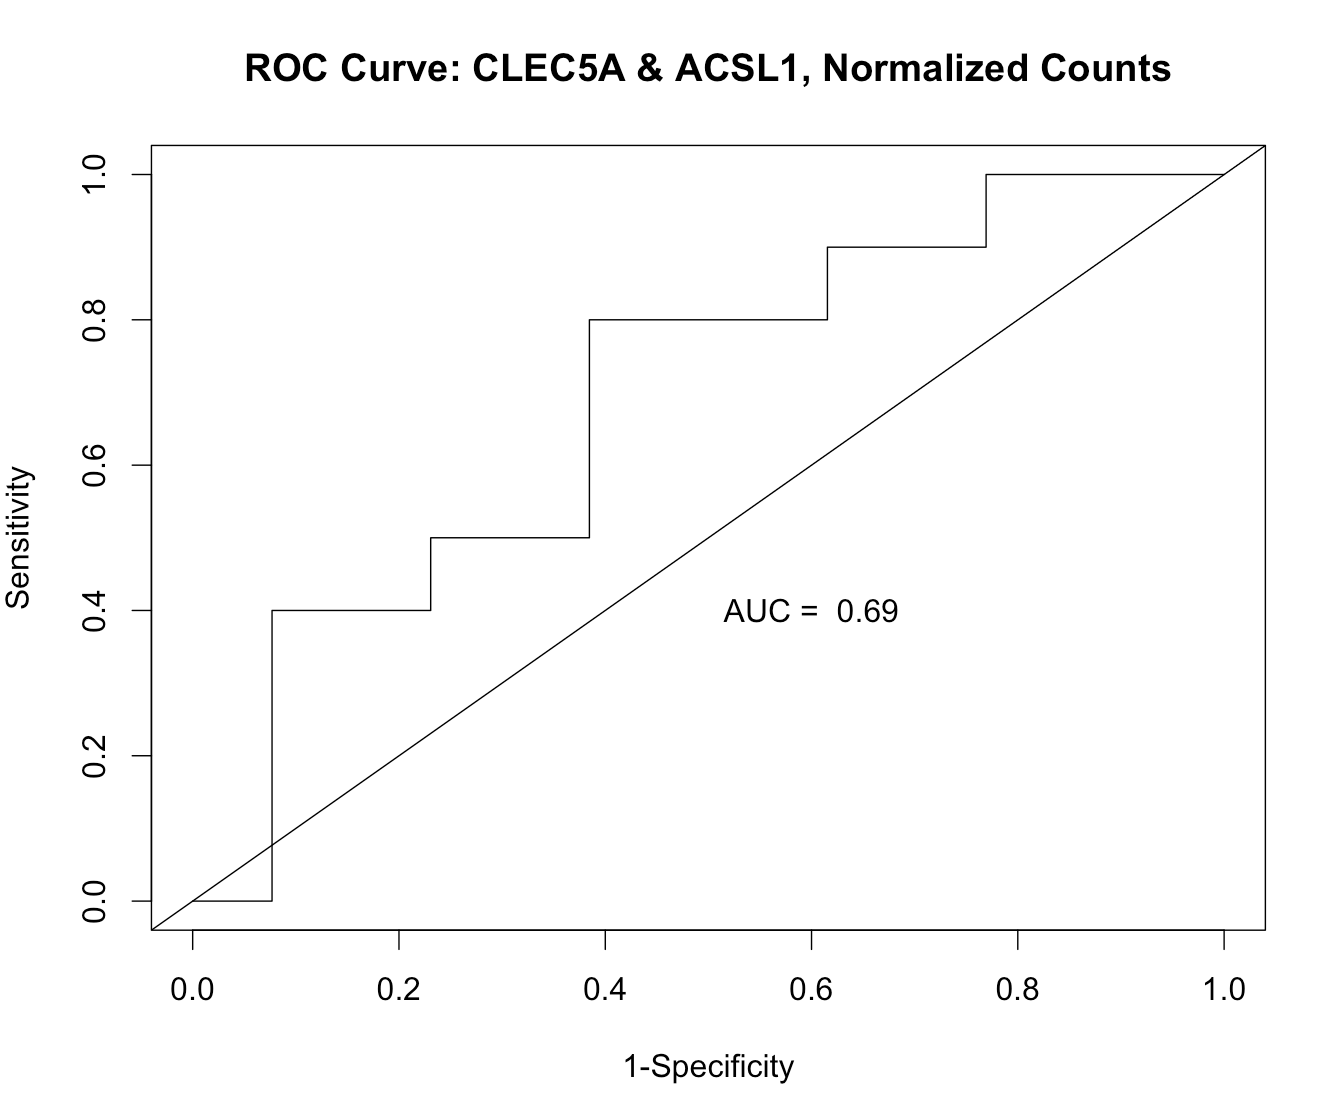
\includegraphics[scale=0.50]{../paper/figs/smoking1.png}
\end{figure}

\begin{figure}[H]
		\centering
		\caption{LASSO PLOT FOR BENZENE}
                 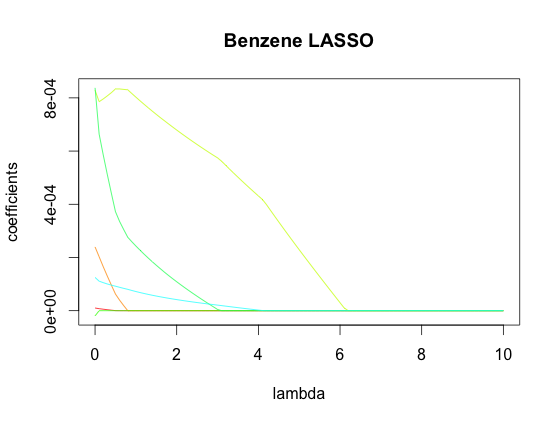
\includegraphics[scale=0.70]{../paper/figs/lasso_coef.png}
\end{figure}

\begin{figure}[H]
		\centering
		\caption{LASSO MEAN SQUARED ERROR FOR BENZENE}
                 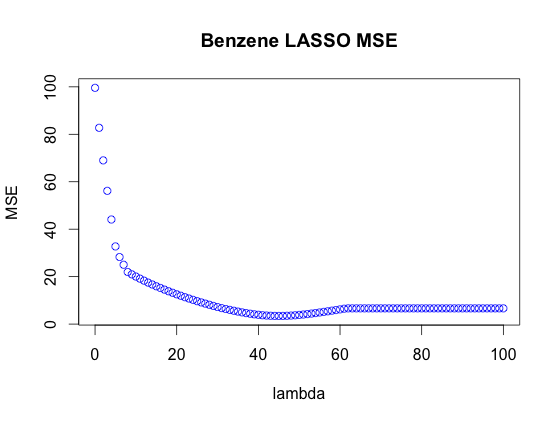
\includegraphics[scale=0.70]{../paper/figs/lasso_mse.png}
\end{figure}


\end{document}
